\documentclass[a4paper, 12pt]{article} % тип документа

%%%Библиотеки
    %\usepackage[warn]{mathtext}	
    \usepackage[T2A]{fontenc}   %Кодировка
    \usepackage[utf8]{inputenc} %Кодировка исходного текста
    \usepackage[english, russian]{babel} %Локализация и переносы
    \usepackage{caption}
    \usepackage{gensymb}
    %\usepackage{listings}
    \usepackage{amsmath, amsfonts, amssymb, amsthm, mathtools}
    %\usepackage[warn]{mathtext}
    %\usepackage[mathscr]{eucal}
    %\usepackage{wasysym}
    %\usepackage{graphicx} %Вставка картинок правильная
    %\usepackage{pgfplots}
    \usepackage{indentfirst}
    %\usepackage{float}    %Плавающие картинки
    %\usepackage{wrapfig}  %Обтекание фигур (таблиц, картинок и прочего)
    \usepackage{fancyhdr}  %Загрузим пакет
    %\usepackage{lscape}
    %\usepackage{xcolor}
    %\usepackage[normalem]{ulem}
    
    \usepackage{titlesec}
    \titlelabel{\thetitle.\quad}

    \usepackage{hyperref}

%%%Конец библиотек

%%%Настройка ссылок
%%%    \hypersetup
%%%    {
%%%        colorlinks = true,
%%%        linkcolor  = blue,
%%%        filecolor  = magenta,
%%%        urlcolor   = blue
%%%    }
%%%Конец настройки ссылок


%%%Настройка колонтитулы
    \pagestyle{fancy}
    \fancyhead{}
    \fancyhead[L]{1.1.1}
    \fancyhead[R]{Засимов Георгий, группа Б01-109}
    \fancyfoot[C]{\thepage}
%%%конец настройки колонтитулы



\begin{document}
                        %%%%Начало документа%%%%


%%%Начало титульника
\begin{titlepage}

    \newpage
    \begin{center}
        \normalsize Московский физико-технический институт \\(национальный исследовательский университет)
    \end{center}

    \vspace{6em}

    \begin{center}
        \Large Лабораторная работа по общему курсу физики\\
    \end{center}

    \vspace{1em}

    \begin{center}
        \Large \textbf{1.1.1. Определение систематических и случайных погрешностей при измерении удельного сопротивления нихромовой проволки}
    \end{center}

    \vspace{2em}

    \begin{center}
        \large Засимов Георгий Алексеевич \\
        Группа Б01-109
    \end{center}

    \vspace{\fill}

    \begin{center}
    Долгопрудный \\2021
    \end{center}
    
\end{titlepage}
%%%Конец Титульника



%%%Настройка оглавления и нумерации страниц
%%%    \thispagestyle{empty}
%%%    \newpage
%%%    \tableofcontents
%%%    \newpage
%%%    \setcounter{page}{1}
%%%Настройка оглавления и нумерации страниц


\textbf{Цель работы:} измерить удельное сопротивление проволоки и вычислить систематические и случайные погрешности при использовании таких измерительных приборов, как линейка, штангенциркуль, микрометр, амперметр, вольтметр и мост постоянного тока.\\

\textbf{Используемое оборудование:} линейка, штангенциркуль, микрометр, отрезок проволоки из нихрома, амперметр, вольтметр, источник ЭДС, мост постоянного тока, реостат, ключ.\\

\textbf{Используются следующие методы измерений сопротивления:} 

1) Определение углового коэффициента наклона зависимости напряжения на проволоке от тока через неё, измеряемых с помощью аналоговых и цифровых вольтметров и амперметров.

2) Измерение с помощью моста постоянного тока. Геометрические размеры образца измеряются с помощью линейки, штангенциркуля и микрометра. Детально исследуется систематические и случайные погрешности проводимых измерений.

В данной работе мы используем оба метода и сравниваем их.\\


\section{Теоретические сведения}

Удельное сопротивленеи проволоки круглого сечения, изготовленного из однородного материала и имеющей всюду одинаковую толщину, может быть определено по формуле
\[\rho = \frac{R_{\text{пр}}}{L} \frac{\pi d^2}{4}\]

В этой формуле $R$ -- сопротивление измеряемого отрезка проволоки, $d$ -- диаметр проволоки, $L$ -- длина отрезка проволоки.

Так как диаметр проволоки флуктуирует в зависимости от места измерения и толщины, необходимо найти среднее значение толщины по всей длине проволоки. Также необходимо учесть погрешность измеренной средней толщины при подсчёте погрешности удельного сопротивления проволоки.

Сопротивление проволоки можно искать с помощью двух различных (очень схожих) электрических схем:
\begin{center}
    {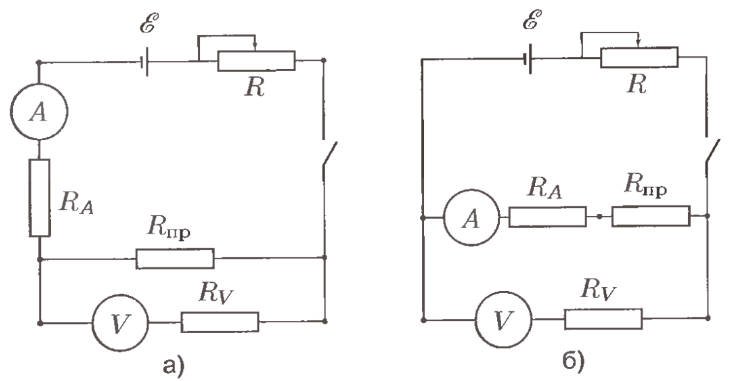
\includegraphics[width=11cm]{1}}
\end{center}

На данных схемах $R_V$ и $R_A$ -- сопротивления вольтметра и амперметра соответственно, а $R$ -- сопротивление реостата.

Для схемы a) имеем:
\[R_{\text{пр1}} = \frac{V_a}{I_a} = R_{\text{пр}} \frac{R_V}{R_V + R_{\text{пр}}} \]

Здесь $R_{\text{пр1}}$ -- измеренное сопротивление проволоки по закону Ома без учёта конечности сопротивления вольметра.

Для схемы б) имеем:
\[R_{\text{пр2}} = \frac{V_{\text{б}}}{I_{\text{б}}} = R_{\text{пр}} + R_A\]

Здесь $R_{\text{пр2}}$ -- измеренное сопротивление проволоки по закону Ома без учёта того, что у амперметра есть сопротивление.

Преобразуем оба выражения:
\[R_{\text{пр}} = R_{\text{пр1}} \frac{R_V}{R_V - R_{\text{пр1}}} = \frac{R_{\text{пр1}}}{1 - (R_{\text{пр1}})/(R_V)} \cong R_{\text{пр1}} (1 + \frac{R_{\text{пр1}}}{R_V})\]

\[R_{\text{пр}} = R_{\text{пр1}} (1 - \frac{R_A}{R_{\text{пр2}}})\]

Естественно, использовтаь надо то выражение, которое даёт меньшую поправку на сопротивление.\\

\section{Используемые оборудование и электрическая схема}

Так как известно, что $R_{\text{пр}}\cong 5$ Ом, оценим по ранее выведенным формулам поправки на сопротивление, учитывая, что $R_V = 10$ МОм и $R_A = 0,5$ Ом:

\[\frac{R_{\text{пр}}}{R_V} = 5 \cdot 10^{-6}, \text{ } \frac{R_A}{R_{\text{пр}}} = 1 \cdot 10^{-1} \Rightarrow \frac{R_{\text{пр}}}{R_V} \ll \frac{R_A}{R_{\text{пр}}}\]

Отсюда делаем вывод, что лучше использовать электрическую схему $a)$, так как она даёт значительно меньшую поправку на сопротивление проволоки.

\begin{center}
\begin{tabular}{|c|c|}
\hline 
Оборудование & Погрешность измерения \\ 
\hline 
Штангенциркуль & 0,05 мм (маркировка производителя) \\ 
\hline 
Микрометр & 0,01 мм (маркировка производителя) \\
\hline 
Вольтметр & $\Delta = (0,003\cdot x + 4k)$, где $x$ -- измер. величина, а $k = 0,1$ мВ \\ 
\hline 
Амперметр & $K\cdot D$, где $K$ -- класс точности, а $D$ -- цена деления \\ 
\hline 
\end{tabular} 
\end{center}

\begin{center}
\begin{tabular}{|c|c|c|}
\hline 
\multicolumn{3}{|c|}{Характеристики амперметра и вольтметра} \\ 
\hline 
Характеристики & Вольтметр & Амперметр \\ 
\hline 
Система & Цифровая & Электромагнитная \\ 
\hline 
Цена деления & 0,1 мВ & 5 мА \\ 
\hline 
Число делений шкалы & - & 150 \\ 
\hline 
Чувствительность & 10000 дел/В & 200 дел/A \\ 
\hline 
Класс точности & - & 0,5 \\ 
\hline 
Предел измерений & 5 В & 750 мА \\ 
\hline 
Внутреннее сопротивление & 10 МОм & 0,5 Ом \\ 
\hline  
\end{tabular} 
\end{center} 
\newpage

\section{Результаты измерений диаметра проволоки}


Составим таблицу на основе измеренных данных толщины проволоки с помощью штангенциркуля и микрометра:

\begin{center}
\begin{tabular}{|c|c|c|c|c|c|c|c|c|c|c|}
\hline 
 & 1 & 2 & 3 & 4 & 5 & 6 & 7 & 8  \\ 
\hline 
$d_{10},$ мм & 0,4 & 0,4 & 0,4 & 0,4 & 0,4 & 0,4 & 0,4 & 0,4\\ 
\hline 
$d_{20},$ мм & 0,36 & 0,36 & 0,37 & 0,37 & 0,36 & 0,355 & 0,355 & 0,36\\ 
\hline 
\end{tabular} 
\end{center}

При измерении диаметра проволоки штангенциркулем случайная погрешность измерений отсутствует. Следовательно, точность результата определяется только точностью штангенциркуля (систематической погрешностью):
\[d_{10} = (0,4 \pm 0,05) \text{ мм}\]

Из полученных значений диаметров следует, что лучше пользоваться микрометром -- он более точный.

Посчитаем среднее значение для $d_{20}$: $\overline{d_{20}} = 0,36125$ мм.

Для погрешностей имеем:
\[\sigma_{\text{сл}2} = \frac{1}{N}\sqrt{\sum_{i = 0}^{n}{(d_i-\overline{d_{20}})^2}} = 1,54\cdot 10^{-3} \text{ мм}\] 
\[\sigma_{\text{сист}2} = 0,01 \text{ мм}\]

Поскольку $\sigma_{\text{сл}2}^2 \ll \sigma_{\text{сист}2}^2$, можно считать. что проволока однородна по диаметру и погрешность фактически определяется систематической:
\[d_{20} = \overline{d_{20}} \pm \sigma_d = (0,36125 \pm 0,01) \text{ мм}\]

Площадь поперечного сечения равна:
\[S = \frac{\pi \overline{d_{20}}^2}{4} = 102,5\cdot 10^{-3}\text{ мм}^{2}\]

Погрешность определим через формулу погрешностей косвенных измерений:
\[\sigma_S = \frac{\partial{S}}{\partial{d}}\sigma_d = \frac{2S}{\overline{d_{20}}}\sigma_d = 5,67\cdot 10^{-3}\text{ мм}^{2}\]\\\\\\

\section{Результаты измерений сопротивления проволоки}

Соберём электрческую схему $a)$ и проводим измерения вольт-амперной характеристики для трёх величин расстояния проволоки:\\ $l_1=(20\pm 0,1)$ см, $l_2=(30\pm 0,1)$ см, $l_3=(50\pm 0,1)$ см

Для большей точности измерения вольт-амперной характеристики проведём при возрастающих и убывающих значениях тока. Все показания приборов заносим в таблицу:
\begin{center}
\begin{tabular}{|c|c|c|c|c|c|c|c|c|}
\hline
\multicolumn{9}{|c|}{Измерение напряжения и силы тока на проволоке}                                                                                \\ \hline
\multicolumn{2}{|c|}{$L = 20$ см} & \multicolumn{2}{c|}{$L = 30$ см} & \multicolumn{2}{c|}{$L = 50$ см}                         \\ \hline
$U$, В & $I$, А & $U$, В & $I$, А & $U$, В & $I$, А \\ \hline
0,4395&0,225&0,6630&0,225&1,0666&0,220 \\ \hline  
0,4991&0,255&0,7710&0,260&1,1646&0,235 \\ \hline
0,5556&0,280&0,9346&0,315&1,3515&0,275 \\ \hline
0,6955&0,350&1,1066&0,370&1,6372&0,330 \\ \hline
0,8105&0,405&1,5501&0,470&2,0074&0,400 \\ \hline
1,1800&0,580&2,2747&0,740&3,2820&0,640 \\ \hline
1,1801&0,580&1,9452&0,635&2,7892&0,550  \\ \hline
0,8260&0,415&1,6787&0,505&2,3468&0,465 \\ \hline
0,7421&0,365&1,2231&0,410&1,8276&0,365 \\ \hline
0,5681&0,290&1,0467&0,350&1,5032&0,305 \\ \hline
0,5164&0,265&0,8342&0,280&1,2345&0,250 \\ \hline
0,4186&0,215&0,6921&0,235&1,1332&0,230 \\ \hline
\end{tabular}
\end{center}

Строим графики зависимостей $U(I)$ для всех для всех трёк длин отрезков проволоки, проводя прямые через экспериментальные точки. Из графиков видно, что нет различия между значениями, полученными при возрастании и при уменьшении тока (нет петли Гистерезиса).

\begin{center}
    {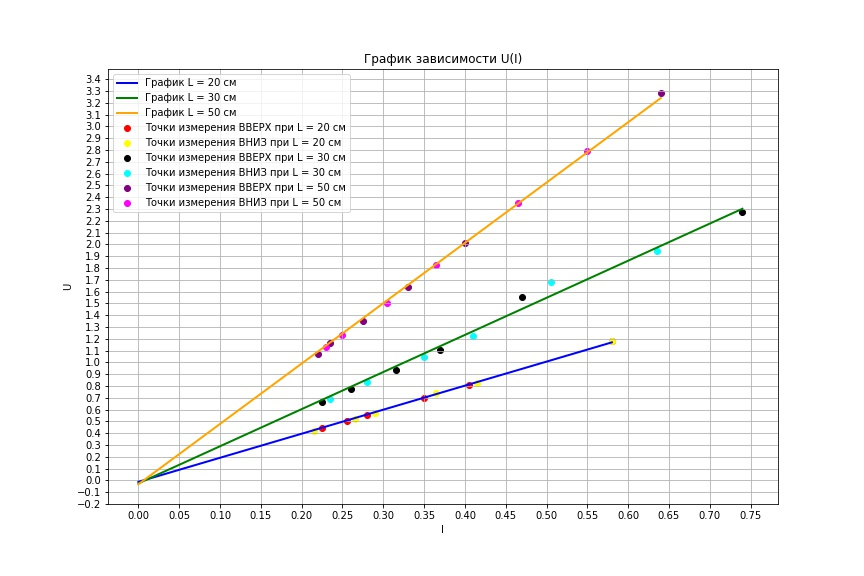
\includegraphics[width=14cm]{schedule}}
\end{center}

Далее снимаем данные сопротивлений пролоки при разных длинах с помощью моста, записываем в таблицу.

По закону Ома $U=RI$ также нужно вспомнить, что погрешность каждого измерения напряжения $\Delta U$ выражается формулой, приложенной в инструкции к вольтметру:
\[\Delta U = (0,003\cdot U + 0,0004)^{3}\]

Рассчитываем все погрешности напряжения и заносим в таблицу. Также вспоминаем, что погрешность амперметра равна $\Delta I = 0,5 \cdot 5$ мА $= 2,5$ мА -- выражается через класс точности и цену деления.

В данном случае лучше воспользовать методом Пирсона (хи-квадрат), чтобы учесть погрешности отдельных измерений напряжения. 

\[R_{\text{ср}} = \frac{\langle VI \rangle '}{\langle I^2 \rangle '}, \text{ } \sigma_{R_{\text{ср}}} = \frac{1}{\sqrt{N}} \sqrt{\frac{\langle U^2 \rangle '}{\langle I^2 \rangle '} - R^2_{\text{ср}}}\]

Для измеренных данных имеем:
\[R_{\text{ср}1} = 2,224 \text{ Ом, }R_{\text{ср}2} = 3,292\text{ Ом, }R_{\text{ср}3} = 5,395\text{ Ом }\]
\[\sigma_{R_{\text{ср}1}} = 0,012 \text{ Ом, }\sigma_{R_{\text{ср}2}} = 0,011\text{ Ом, }\sigma_{R_{\text{ср}3}} = 0,010\text{ Ом }\]

Данные сопротивлений проволоки, снятые с помощью моста, имеют вид:
\[R_{\text{мост}1} = 2,211 \text{ Ом, }R_{\text{мост}2} = 3,281\text{ Ом, }R_{\text{мост}3} = 5,386\text{ Ом }\]

Видим, что данные сопротивлений, свнятые с помощью моста и с помощью схемы примерно совпадают.

В нашем случае $N = 12$ -- число экспериментальных точек. Погрешность амперметра равна
\[\sigma_I = 0,5 \cdot 5 \text{ мА} = 2,5 \text{ мА}\]

В методе хи-квадрат мы воспользовались погрешностями напряжений, теперь учтём и погрешность амперметра:

\[\sigma_{R_{\text{полн}}} = \sqrt{ \left(\frac{\partial R}{\partial I} \sigma_I\right)^2 + \sigma_{R_{\text{ср}}}^2} = \sqrt{ \left(\frac{R_{\text{ср}}}{I} \sigma_I\right)^2 + \sigma_{R_{\text{ср}}}^2}\]

Для оценки погрешности возьмём предел измерений силы тока $I =$ $0,750$ А.

Отсюда получаем следующие значения погрешностей:
\[\sigma_{R_{\text{полн}1}} = 0,014 \text{ Ом, }\sigma_{R_{\text{полн}2}} = 0,016\text{ Ом, }\sigma_{R_{\text{полн}3}} = 0,021\text{ Ом }\]

Не забываем внести поправку в значения сопротивлений с помощью формулы:

\[R_{\text{пр}} = R_{\text{полн}} (1 + \frac{R_{\text{полн}}}{R_V})\]

Так как попроавка очень мала (даже слишком), можно считать, что $R_{\text{пр}} = R_{\text{полн}}$ и $\sigma_{R_{\text{пр}}} = \sigma_{R_{\text{полн}}}$.

Для удобства составим таблицу погрешностей измерения сопротивлений:
\begin{center}
\begin{tabular}{|c|c|c|c|}
\hline 
$L$, см & 20 & 30 & 50 \\ 
\hline 
$R_{\text{полн}}$, Ом & $2,224$ & $3,292$ & $5,395$ \\ 
\hline 
$R_{\text{пр}}$, Ом & $2,224$ & $3,292$ & $5,395$ \\ 
\hline 
$\sigma_{R_{\text{полн}}}$, Ом & $0,014$ & $0,016$ & $0,021$ \\ 
\hline 
$\sigma_{R_{\text{пр}}}$, Ом & $0,014$ & $0,016$ & $0,021$ \\ 
\hline 
$\sigma_{R_{\text{мост}}}$, Ом & $2,211$ & $3,281$ & $5,386$ \\ 
\hline  
\end{tabular} 
\end{center}
\newpage
\begin{center}
 \textbf{Обработка данных для поиска удельного сопротивления проволоки}
\end{center}

Удельное сопротивление проволоки и его погрешность определяются формулами:
\[\rho = \frac{R_{\text{пр}}}{L} \frac{\pi \overline{d_{20}}^2}{4}, \text{ } \sigma_{\rho} = \rho \sqrt{\Big( \frac{\sigma_{R_{\text{пр}}}}{R_{\text{пр}}}\Big) ^2 + \Big(\frac{\sigma_S}{S} \Big)^2 + \Big(\frac{\sigma_L}{L} \Big)^2}\]

Здесь $\sigma_{L} = 0,1$ см.
Занесём все результаты в таблицу:
\begin{center}
\begin{tabular}{|c|c|c|c|}
\hline 
$L$, см & 20 & 30 & 50 \\ 
\hline 
$\rho \cdot 10^{-5}$, Ом$\cdot$см & $8,69$ & $8,57$ & $8,43$ \\ 
\hline 
$\sigma_{\rho}\cdot 10^{-6}$, Ом$\cdot$см & $4,93$ & $4,84$ & $4,74$ \\ 
\hline 
\end{tabular} 
\end{center}

\section{Выводы}

Измерили удельное сопротивление проволоки и вычислили систематические и случайные погрешности при использовании таких измерительных приборов, как линейка, штангенциркуль, микрометр, амперметр, вольтметр и мост постоянного тока.



\end{document}